%%%%%%%%%%%%%%%%%%%%%%%%%%%%%%%%%%%%%%%%%%%%%%%%%%%%%%%%%%%%%%%%%%%%%%%%%%%%
% AGUtmpl.tex: this template file is for articles formatted with LaTeX2e,
% Modified July 2014
%
% This template includes commands and instructions
% given in the order necessary to produce a final output that will
% satisfy AGU requirements.
%
% PLEASE DO NOT USE YOUR OWN MACROS
% DO NOT USE \newcommand, \renewcommand, or \def.
%
% FOR FIGURES, DO NOT USE \psfrag or \subfigure.
%
%%%%%%%%%%%%%%%%%%%%%%%%%%%%%%%%%%%%%%%%%%%%%%%%%%%%%%%%%%%%%%%%%%%%%%%%%%%%
%
% All questions should be e-mailed to latex@agu.org.
%
%%%%%%%%%%%%%%%%%%%%%%%%%%%%%%%%%%%%%%%%%%%%%%%%%%%%%%%%%%%%%%%%%%%%%%%%%%%%
%
% Step 1: Set the \documentclass
%
% There are two options for article format: two column (default)
% and draft.
%
% PLEASE USE THE DRAFT OPTION TO SUBMIT YOUR PAPERS.
% The draft option produces double spaced output.
%
% Choose the journal abbreviation for the journal you are
% submitting to:

% jgrga JOURNAL OF GEOPHYSICAL RESEARCH
% gbc   GLOBAL BIOCHEMICAL CYCLES
% grl   GEOPHYSICAL RESEARCH LETTERS
% pal   PALEOCEANOGRAPHY
% ras   RADIO SCIENCE
% rog   REVIEWS OF GEOPHYSICS
% tec   TECTONICS
% wrr   WATER RESOURCES RESEARCH
% gc    GEOCHEMISTRY, GEOPHYSICS, GEOSYSTEMS
% sw    SPACE WEATHER
% ms    JAMES
% ef    EARTH'S FUTURE
% ea    EARTH AND SPACE SCIENCE
%
%
%
% (If you are submitting to a journal other than jgrga,
% substitute the initials of the journal for "jgrga" below.)

\documentclass[draft,jgrga]{agutex2015}
% To create numbered lines:

% If you don't already have lineno.sty, you can download it from
% http://www.ctan.org/tex-archive/macros/latex/contrib/ednotes/
% (or search the internet for lineno.sty ctan), available at TeX Archive Network (CTAN).
% Take care that you always use the latest version.

% To activate the commands, uncomment \usepackage{lineno}
% and \linenumbers*[1]command, below:

 \usepackage{lineno}
 \linenumbers*[1]
%  To add line numbers to lines with equations:
%  \begin{linenomath*}
%  \begin{equation}
%  \end{equation}
%  \end{linenomath*}
%%%%%%%%%%%%%%%%%%%%%%%%%%%%%%%%%%%%%%%%%%%%%%%%%%%%%%%%%%%%%%%%%%%%%%%%%
% Figures and Tables
%
%
% DO NOT USE \psfrag or \subfigure commands.
%
%
%  Uncomment the following command to include .eps files
%  (comment out this line for draft format):
%%  \usepackage[dvips]{graphicx}
\usepackage[dvipdfmx]{graphicx}
\usepackage{mediabb}
%\usepackage{here}
%
%  Uncomment the following command to allow illustrations to print
%   when using Draft:
  \setkeys{Gin}{draft=false}
%
% Substitute one of the following for [dvips] above
% if you are using a different driver program and want to
% proof your illustrations on your machine:
%
% [xdvi], [dvipdf], [dvipsone], [dviwindo], [emtex], [dviwin],
% [pctexps],  [pctexwin],  [pctexhp],  [pctex32], [truetex], [tcidvi],
% [oztex], [textures]
%
% See how to enter figures and tables at the end of the article, after
% references.
%
%% ------------------------------------------------------------------------ %%
%
%  ENTER PREAMBLE
%
%% ------------------------------------------------------------------------ %%

% Author names in capital letters:
\authorrunninghead{USUI ET AL.}

% Shorter version of title entered in capital letters:
\titlerunninghead{ELECTRON DYNAMICS IN MINI-MAGNETOSPHERE}

%Corresponding author mailing address and e-mail address:
\authoraddr{Corresponding author: H. Usui,
Graduate School of System Informatics, 
Kobe University, 1-1 Rokkoudai-cho Nada-ku, Kobe, 657-8501, JAPAN
(h-usui@port.kobe-u.ac.jp)}

\begin{document}

%% ------------------------------------------------------------------------ %%
%
%  TITLE
%
%% ------------------------------------------------------------------------ %%


\title{
Electron dynamics in the %boundary layer current of a
 mini-magnetosphere above a lunar magnetic anomaly
}
%

%% ------------------------------------------------------------------------ %%
%
%  AUTHORS AND AFFILIATIONS
%
%% ------------------------------------------------------------------------ %%


%Use \author{\altaffilmark{}} and \altaffiltext{}

% \altaffilmark will produce footnote;
% matching \altaffiltext will appear at bottom of page.

 \authors{
 Hideyuki Usui,\altaffilmark{1}
 Yohei Miyake,\altaffilmark{2}
 Masaki Nishino\altaffilmark{3} 
 Takuma Matsubara,\altaffilmark{1}, and 
 Joseph Wang\altaffilmark{4}}

% \authors{A. B. Smith,\altaffilmark{1}
% Eric Brown,\altaffilmark{1,2} Rick Williams,\altaffilmark{3}
% John B. McDougall\altaffilmark{4}, and S. Visconti\altaffilmark{5}}

\altaffiltext{1}{
Graduate School of System Informatics,
Kobe University, Kobe, Hyogo, Japan
}

\altaffiltext{2}{
Education Center for Computational Science and Engineering, 
Kobe University, Kobe, Hyogo, Japan
}

\altaffiltext{3}{
Institute for Space-Earth Environment Research, Nagoya University, 
Nagoya, Aichi, Japan
}

\altaffiltext{4}{
Department of Astraunautical Engineering, The University of Southern California,
Los Angeles, California, USA.
}

%% ------------------------------------------------------------------------ %%
%
%  KEYPOINTS
%
%% ------------------------------------------------------------------------ %%
% Key points are 1 to 3 points that the author provides,
% that are 100 characters or less, that are ultimately published
% with the article.
%% for example:
% \keypoints{\item Here is the first keypoint. what happens if it is a
% long keypoint, like this one. We want to see this wrap please.
% \item This is the second.
% \item And here is the third keypoint
% }

\keypoints{
\item Boundary layer current in a mini-magnetosphere has a structure of electron turn-around flux
\item Maximum electron velocity at the inner most edge of the magnetosphere is due to the cyclotron motion of accelerated electrons
\item The width of the boundary layer current corresponds to the radius of the local cyclotron motion of electrons
}

%% Keypoints will print underneath the abstract.
%% ------------------------------------------------------------------------ %%
%
%  ABSTRACT
%
%% ------------------------------------------------------------------------ %%

% >> Do NOT include any \begin...\end commands within
% >> the body of the abstract.

\begin{abstract}
We present a three-dimensional 
electromagnetic particle-in-cell 
simulation study of the electron dynamics in the boundary layer current 
of a mini-magnetosphere created above a magnetic anomaly 
on the lunar surface. %by performing three-dimensional 
%electromagnetic particle-in-cell simulations.
The size of the magnetic anomaly (characterized 
by the distance from the center of the magnetic dipole 
to the position where the pressure of the local magnetic field 
equals the dynamic pressure of the solar wind)
considered here is about four times smaller than the 
 Larmor radius of the solar wind ions. 
%can be characterized 
%by the distance $L$ from the center of the magnetic dipole 
%to the position where the pressure of the local magnetic field 
%becomes equal to the dynamic pressure of the solar wind. 
%In the case where the Larmor radius of the solar wind ions is 
%four times larger than $L$, 
We find that a mini-magnetosphere 
is formed with asymmetric density profiles. 
It is shown that the boundary layer current is dominated 
by the electron flux.
As an intense electric field is induced 
in the boundary layer by the charge separation between 
electrons and ions, the electrons entering the boundary layer 
%start making 
undergo the $E\times B$ drift motion in the equator. 
In the high latitude region, on the other hand, the electron flux 
turns around and the direction of the electron motion  %%is this what you mean
becomes reversed. 
This causes a turn-around current in each hemisphere. 
We also examine the detail of the electron dynamics in the equator 
in terms of electron cyclotron motion. 
It is shown that the maximum electron velocity observed 
at the inner most edge of the magnetosphere is due to 
the electron cyclotron motion itself rather than the drift motion of 
the electrons’ guiding center. 
We also confirm that the width of the boundary layer current is 
approximately equal to the radius of the local electron cyclotron motion.
%%(248 words)
\end{abstract}

%% ------------------------------------------------------------------------ %%
%
%  BEGIN ARTICLE
%
%% ------------------------------------------------------------------------ %%

% The body of the article must start with a \begin{article} command
%
% \end{article} must follow the references section, before the figures
%  and tables.

\begin{article}

%% ------------------------------------------------------------------------ %%
%
%  TEXT
%
%% ------------------------------------------------------------------------ %%

\section{Introduction}
The lunar plasma environment has been  investigated 
intensively by recent spacecraft observations  such as
KAGUYA \citep[e.g.][]{Saito2008,Saito2010,Saito2012} and
Chandrayaan-1 \citep[e.g.][]{Barabash2009,Bhardwaj2010}.
In addition to the macroscopic plasma structure
such as the wake structure formed in the downstream region,
small-scale perturbations of plasma distribution and fields were also
 observed in the dayside region,
mostly over the crustal magnetic anomalies found on the lunar surface.
KAGUYA spacecraft observed
more than $10 \%$ of the solar wind protons reflected at the altitude around 100km
over the magnetic anomalies (\cite{Saito2010}).
Chandrayaan-1 found the deflection of the solar wind protons with
a high efficiency of more than $ 10 \%$ (\cite{Lue2011}) and
also observed the backstreaming hydrogen atoms over the magnetic anomalies (\cite{Wieser2010}).
In association with the plasma variation,
plasma wave activities are also enhanced over the magnetic anomalies
\citep[e.g.][]{Halekas2006a,Hashimoto2010}.
These observations suggest that the plasma and field disturbances over
the magnetic anomalies are caused by the solar wind interactions
with the local magnetic fields.
Unlike the Earth's magnetosphere, %however, 
the dipole moment of
the lunar magnetic anomalies is very weak and
the resulting dipole field region is much smaller than the characteristic spatial scales
of the solar wind, such as the ion inertial length and the ion's Larmor radius $r_\mathrm{iL}$.



We define  the typical spatial scale of a magnetic dipole $L$ 
as the distance from the center of the magnetic dipole 
to an equilibrium point 
where the plasma dynamic pressure under the magnetohydrodynamics (MHD) approximation 
balances  the local magnetic pressure of the dipole field.
For lunar magnetic anomalies,
$L$ can be less than 100km and smaller than $r_\mathrm{iL}$.
In such a situation,
the protons are almost unmagnetized and their dynamics are not affected significantly 
by the local field of magnetic anomalies.
However, as stated above,
a variety of ion dynamics phenomena such as the ion reflection and deflection have been observed.
The mechanism underlying the ion dynamics above the magnetic anomalies is thought to relate
to the solar wind interactions with the magnetic anomalies.
%%%Hide, is this what you want to say here??

The interactions between a plasma flow and a small-scale magnetic dipole 
have been examined in different situations.
When $L$ is comparable to or smaller than $r_\mathrm{iL}$
but larger than the electron Lamor radius $r_\mathrm{eL}$,
this spatial range is called the meso-scale.
In one of the feasibility studies of a future interplanetary flight system called magneto-sail,
the solar wind interactions with a meso-scale magnetic dipole artificially created by a
superconducting coil equipped at a spacecraft was examined using two-dimensional
particle-in-cell (PIC) plasma simulations (\cite{Moritaka2012}).
That study showed the formation of a magnetosphere even in a meso-scale regime.
In the interactions between the solar wind and a meso-scale magnetic dipole,
the electrons are magnetized while ions are less magnetized at the magnetopause.
An electric field is induced at the dayside magnetosphere by charge separation
due to the momentum difference between the electrons and ions.
It was shown that the electric field induced at the magnetopause
can affect the dynamics of the incoming solar wind ions and some of the ions can be reflected
back to the sunward direction.

A similar interaction takes place between the solar wind and the lunar magnetic anomalies.
A mini-magnetosphere with a density cavity has been studied both by
 spacecraft observations and numerical simulations
\citep[e.g.][]{Harnett2000,Harnett2003,Halekas2008b,Bamford2012}.
The plasma responses to the induced electric field were also examined
in  previous particle simulation studies
\citep[e.g.][]{Harnett2002,Kallio2012,Poppe2012a,Deca2014,Deca2015}.
Laboratory experiments on plasma interactions
with a small-scale magnetic dipole
were also conducted and the electric field 
induced by the interaction
between a plasma flow and the local magnetic fields were examined
\citep[e.g.][]{Howes2015,Jarvinen2014,Wang2013,Bamford2012}.
%-- comment by referee2---
The solar wind interaction with a real magnetic anomaly was also 
examined with hybrid particle simulation 
\citep{Fatemi2015}.
%-----


As pointed out in many previous studies,
plasma kinetics such as the  finite Larmor radius effect should be included in modeling
the interactions between the solar wind and the magnetic anomalies
because $L$ is almost the same as or smaller than $r_\mathrm{iL}$.
The electric field generated by
the charge separation  at the magnetopause affects 
the dynamics of the solar wind ions. %  affected and some of them are reflected.
Meanwhile, the solar wind electrons are  magnetized in the mini-magnetosphere.
Hence, the boundary layer current is mainly due to the electron flux.
It is reported that the electrons in the boundary layer of the mini-magnetosphere 
mainly make a drift motion with the $E \times B$ velocity.
The electron dynamics in terms of velocity distribution function at different locations above
the magnetic anomaly were examined in \cite{Deca2015}.
However, the detail of the three-dimensional structure of the boundary layer current,
which is  dominated by the electron flux, has not been studied yet.

In this study,
we study the spatial structure of the boundary layer current 
in a mini-magnetosphere formed above a lunar magnetic anomaly
using  three-dimensional electromagnetic particle-in-cell simulations.
The simulation results presented focus on the electron dynamics in the boundary layer.
In Section II, we describe the simulation model used in this study.
In our model we adopted a case of $r_\mathrm{iL} /L=4$ for the magnetic anomaly.
In Section III, we show the spatial variation of plasma density and the current density
by cutting different planes out of the three-dimensional space in the simulations.
In addition to the asymmetric density profiles of a mini-magnetosphere created above
the magnetic anomaly, 
we also examine the three-dimensional structure of the boundary layer current.
In Section IV, we discuss the electron dynamics on the equatorial plane in detail
particularly at the most inner edge of the mini-magnetosphere 
where the electron density decreases to zero.
Finally we summarize the results and present the conclusion in Section V.


\section{Methods}
This study is based on three-dimensional, full kinetic,
electromagnetic particle-in-cell simulations.
In the simulation, Reiner Gamma, 
which is one of the typical magnetic anomalies on the lunar surface, 
is refereed to as a model of magnetic anomaly. 
In the case of Reiner Gamma, 
the magnetic dipole moment is almost parallel to the lunar surface. 
The dipole center is approximately located at a depth of 10 km under the ground. 
The amount of the dipole moment is $1.123 \times 10^{13} Am^2$.

%% - Figure 1-
\begin{figure}[t]
 \centering
%\noindent\includegraphics[width=12cm]{./Fig_1_bb-crop.pdf}
%\noindent\includegraphics[width=8cm]{./figures/Fig_1_bb-crop.pdf}
 \noindent\includegraphics[]{./figures/Fig_1_bb-crop.pdf}
 \caption{(a) Three-dimensional simulation model, (b) $x-z$ plane, (c) $x-y$ plane}\label{fig:1}
\end{figure}

%% - Table 1-
\begin{table}[h]
\caption{Typical values of the upstream plasma and the magnetic dipole}
%typical real parameters
\centering
 \begin{tabular}{p{16zw}ll}
 Parameters of upstream plasma    &  Notations    &  Typical values \\  \hline           
 Mass ratio between ion and electron & $m_\mathrm{i}/m_\mathrm{e}$ & 1837 \\
 Density       & $n_\mathrm{e}$, $n_\mathrm{i}$  &  $3.5 \times 10^6 \mathrm{m^{-3}}$   \\ 
 Flow velocity & $v_\mathrm{flow}$               &  $400  \mathrm{km/s}  $              \\
 Mach number   & $M_\mathrm{A}$                  & 10.0 \\
 Beta          &  $\beta$                        & 0.96 \\
 Plasma temperature & $T_\mathrm{e}$, $T_\mathrm{i}$    &  $8.6$ eV \\
 Ratio between electron cyclotron frequency and plasma frequency & 
  $\Omega_\mathrm{ce}/\omega_\mathrm{pe}$ & $5.83 \times 10^{-3}$ \\ 
 Uniform magnetic field density &  $B_\mathrm{0}$   &   3.5 nT          \\ \hline 
                &                                &     \\
 Parameters of magnetic dipole               &                &         \\ \hline
 Magnetic moment &  $ m_\mathrm{a}$   &  $ 1.123 \times 10^{13} \mathrm{Am^2}$ \\
 Distance between the dipole center and the lunar surface & $L_\mathrm{surface}$ & 11 km \\
 Balance point between the B-field energy and plasma dynamic pressure 
 & $L$ &  32 km  from the dipole center  \\
 Magnetic field density at $L$  & $B_\mathrm{L}$ & 34.3 nT  \\  \hline
 \end{tabular}
\end{table}


%% - Table 2-
\begin{table}[h]
\caption{
Simulation parameters
}
\centering
 \begin{tabular}{p{16zw}ll}
 Parameters    &  Notations    &  Values \\  \hline           
 Mass ratio between ion and electron & $m_\mathrm{i}/m_\mathrm{e}$    & 100 \\
 Mach number                         & $M_\mathrm{A}$ & 5.0 \\
 Flow velocity                       & $v_\mathrm{flow} $  &  $0.05v_\mathrm{c}$ \\
 Electron thermal velocity           & $v_\mathrm{the}$ &  $0.12v_\mathrm{c}$ \\
 Ion thermal velocity                & $v_\mathrm{thi}$ &  $ 0.012v_\mathrm{c}$ \\
 Ratio between electron cyclotron frequency and plasma frequency & 
  $\Omega_\mathrm{ce}/\omega_\mathrm{pe}$ & 0.1 \\  \hline

 Numbers of grids in the physical region  &  
 $N_x \times N_y \times N_z$        &  $192 \times 192 \times 192$  \\
 System dimensionts                 &   
$l_x \times l_y \times l_z$ & $ 5.6L \times 5.6L \times 5.6L$  \\
 Grid size                          &   $dr$  & $1.0\lambda_\mathrm{D}$  \\
 Time step                          &   $dt$  &  $0.285dr/v_\mathrm{c}$  \\
 Ratio between the ion Larmor radius and $L$ &
     $ r_\mathrm{iL}/L$  & 4 \\
 Location of the dipole moment under the lunar surface  &   $L_\mathrm{surface}$ 
 &  0.2$L$ \\   \hline
 \end{tabular}
\end{table}


%%%%%%%%%%%%%%%%%%%%%%%
Figure \ref{fig:1} shows a three-dimensional simulation model.
In Table 1, we list the simulation parameters used in the simulation. 
In the positive $x$ direction, 
we have a plasma flow representing the solar wind 
with the velocity $v_\mathrm{flow}$. 
The static magnetic field representing the interplanetary magnetic fields (IMF) 
is also introduced in the simulation domain. 
In this study, the IMF direction is northward. 
The Mach number $M$ which is a ratio of $v_\mathrm{flow}$ to 
the Alfv\'{e}n velocity $v_\mathrm{A}$ is 5. 
The values used for the plasma flow parameters are as follows. 
Instead of using actual measured physical values, 
we used scaled ones to reduce the calculation time. 
We set the mass ratio between ion and electron as $ m_\mathrm{i}/ m_\mathrm{e}$ = 100. 
We set the ratio of the speed of light $v_\mathrm{c}$ to $v_\mathrm{flow}$ to be 20, 
although the actual ratio is about 600. 
The plasma flow is isothermal and 
the ratio of the electron thermal velocity 
$v_\mathrm{the}$ to $v_\mathrm{flow}$ is set to be 2.4, 
which is almost the same as the actual ratio for the solar wind electrons. 
The beta value and the ratio of the electron plasma frequency to 
the electron cyclotron frequency,
$\omega_\mathrm{pe} / \Omega_\mathrm{e}$, 
in the solar wind are set be a unity and 10, respectively. 

The  simulation domain consists of $256 \times 256 \times 256$ grids. 
The length of each side of the domain is approximately $7.168L$. 
The electromagnetic perturbation propagating out of the simulation region
are attenuated in the absorbing regions arranged on all of the outer boundaries. 
The width of the field absorbing region is 32 grids.
The grid size $dr$ corresponds to $\lambda_\mathrm{D}$, 
where $\lambda_\mathrm{D}$ denotes the Debye length in the solar wind plasma.
The physical region surrounded by the field absorbing regions consists of 
$192 \times 192 \times 192$ grids. 
The time increment $dt$ was chosen to satisfy 
the Courant condition, $dx/dt > 1.73 v_\mathrm{c}$, in three dimensions. 
The plasma flow typically consists of $5.37 \times 10^8 $ macroparticles in the simulation space. 
We have the lunar surface which is a $yz$ plane placed 
at the right side of the simulation domain.
Under the surface, we set an ideal dipole magnetic field with 
a magnetic moment $M$ which is arranged along the $z$ direction. 
The ratio of $L_\mathrm{surface}$ to $L$ is set to be 0.2, 
where $L_\mathrm{surface}$ denotes
the distance from the dipole field center to the lunar surface.
The dipole magnetic field is considered in the equation of motion 
when the velocity of each particle is updated. 
In the simulations, 
we initially load the solar wind plasma uniformly with $v_\mathrm{flow}$
and continue to inject the plasma flow from the left boundary of the simulation region
toward the lunar surface.
Particles crossing the lunar surface or the other simulation boundaries are 
eliminated from the calculation. 
At the lunar surface, these particles velocities are counted as the electric current and 
contribute to the update of the electric field at each time step at the lunar surface. 
The electric field at the lunar surface corresponds to the surface charging.
For simplicity, we assume no photoelectron emissions from the surface. 

\section{Simulation Results}

%% - Figure 2-
\begin{figure}[t]
\centering
\noindent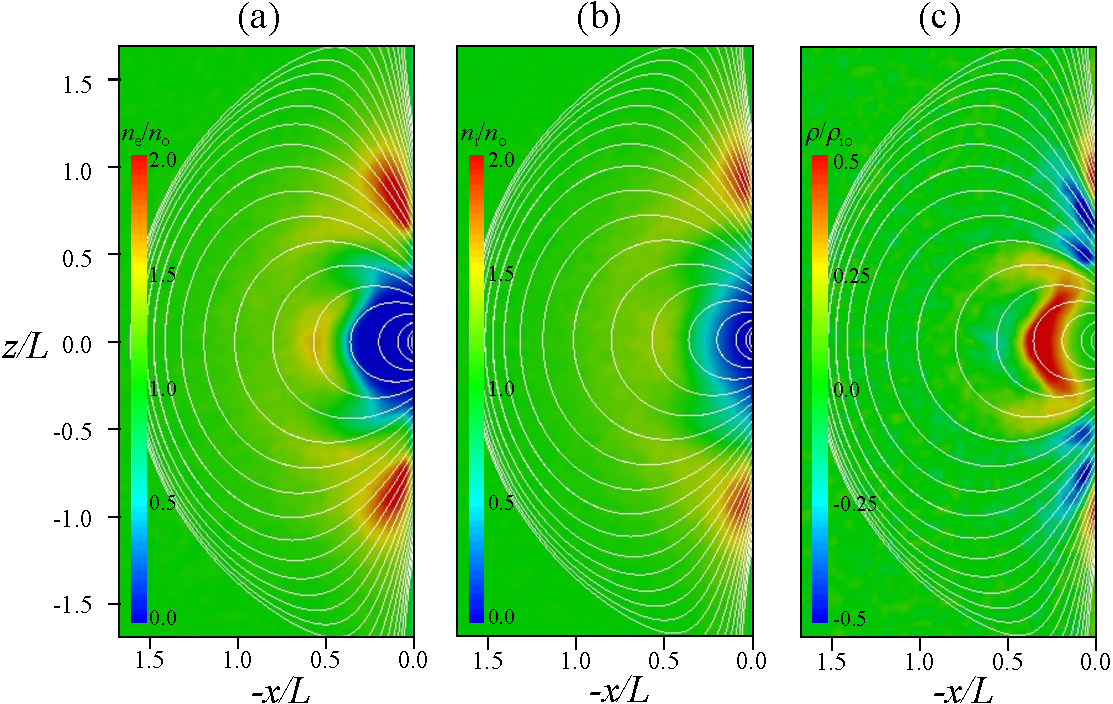
\includegraphics[width=15cm]{./figures/Fig_2_bb-crop.pdf}
\caption{Conour maps of electron and ion densities and the charge density 
obtained at the steady state in a meridian plane}\label{fig:2}
\end{figure}

First we examine the density profiles to see 
if a mini-magnetosphere is created as a result of 
the solar wind interaction with the magnetic anomaly.
Figure \ref{fig:2} shows contour maps of the number densities of electrons and ions  
and the charge density obtained at the steady state 
in the meridian plane which includes $y/L = 0$, respectively. 
Note that $x/L=0$ represents the lunar surface and 
the origin of the coordinate is located at the center of the lunar surface.
We have a solar wind flow from the left to the right direction. 
The absolute values of the $x$ axis implies the altitude from the lunar surface.
As shown in the panels, a mini-magnetosphere with a plasma cavity is clearly 
created above the magnetic anomaly, 
which were studied in the previous works such as
\citep[e.g.][]{Harnett2000,Harnett2003,Halekas2008b,Bamford2012}.
The size of the mini-magnetosphere is less than $0.5L$.
In panel (a) which shows the electron density profile, 
it is found that the boundary of the mini-magnetosphere is curved 
into an arc-shape which corresponds to the dipole fields structure.
It is also found that there is a sharp transition to 
the electron cavity region in the inner magnetosphere. 
For example, 
the density transition is found at $-x/L = 0.3$ 
along the line of $z/L =0$ in panel (a).
We also notice that the density becomes relatively high 
in the high latitude regions around
$|z|/L=0.8$ between the lunar surface and $-x/L=0.3$.
These regions correspond to the cusps where the dipole fields converge to the poles.
In panel (b) indicating the ion density, 
we also confirm the formation of the mini-magnetosphere as shown in panel (a) for electrons.
However, 
the density gradient at the boundary of the mini-magnetosphere is 
not as high as that of electrons.
Across the line of the density transition found in panel (a), 
some ions reach the inner magnetosphere because of large inertia of ions. 
In addition, the mini-magnetosphere itself seems compressed toward the lunar surface.
The ion density becomes also relatively high in the high latitude regions 
where the high density of electrons is found. 
In comparison between panels (a) and (b), 
the spatial profiles of the mini-magnetosphere are overall similar to each other. 
However, because of some differences in the density profiles as stated above, 
we found a spatial variation in terms of charge density as shown in panel (c). 
Panel (c) shows that ions are rich in the low latitude region 
within $|z|/L$ = 0.5 in the inner magnetosphere as shown in red region. 
In the high latitude regions between $|z|/L \sim 0.5$ to 1.0 near the lunar surface, 
however, electrons are relatively rich as shown in blue in panel (c).

% -- up here at the library in USC 2015/12/4 pm 4

%% - Figure 3-
\begin{figure}[t]
\centering
\noindent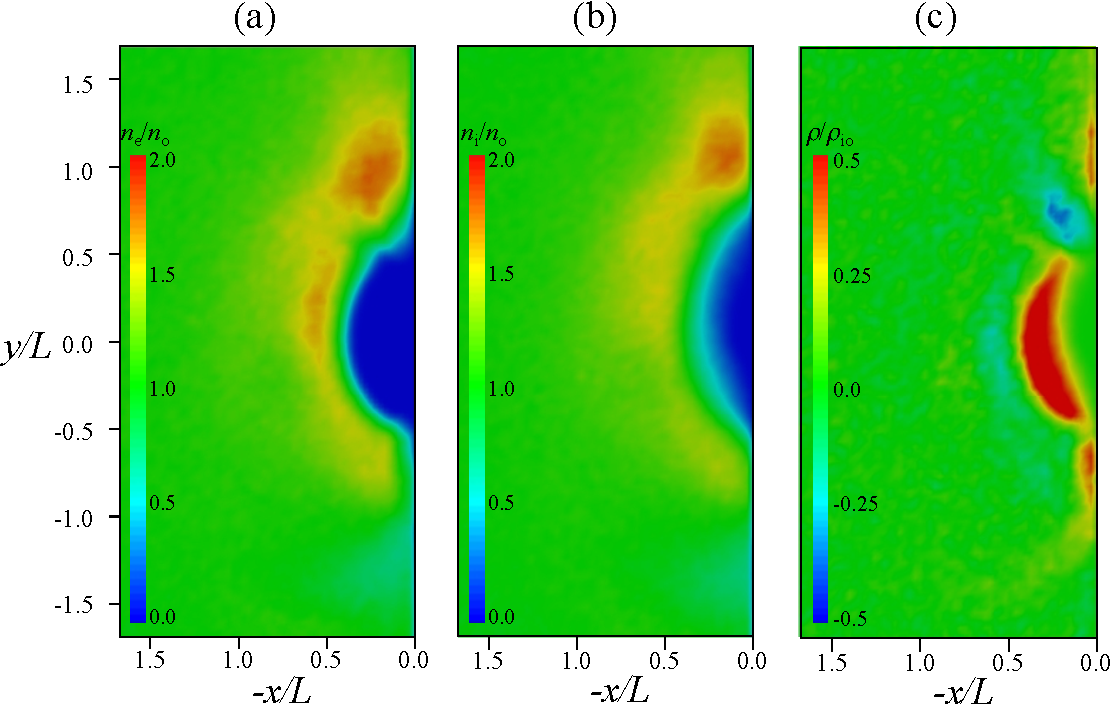
\includegraphics[width=15cm]{./figures/Fig_3_bb-crop.pdf}
\caption{Conour maps of electron and ion densities and the charge density 
obtained at the steady state in the equatorial plane}\label{fig:3}
\end{figure}

Figure \ref{fig:3} shows contour maps of the number densities 
for electrons and ions and the charge density in the equatorial plane 
in the same manner as shown in Figure \ref{fig:2}. 
One of the interesting features we notice in the figure is 
asymmetric density profile of the outer magnetosphere 
with respect to the line of $y/L =0$.
As shown in panels (a) and (b), a high density region is created 
both for electrons and ions in the upper region of the panel
which corresponds to the dawnside region of the outer magnetosphere. 
The profile of the charge density shown in panel (c) is overall 
similar to that in panel (c) of Figure \ref{fig:2}. 
Since ions which have larger inertia than electrons can reach the inner magnetosphere, 
an ion rich region shown in red is created mostly 
along the inner boundary of the mini-magnetosphere. 
Similar to the profiles in panels (a) and (b), 
the charge density profile also has an asymmetric profile shown in panel (c). 
In the dawnside region around $y/L = 0.5$ to 1.0, however, 
an electron rich region is locally created near the lunar surface shown in blue. 
These plasma responses to the magnetic anomaly 
including the formation of a mini-magnetosphere and 
the asymmetric profile of the plasma density have been investigated 
by the previous studies such as
\citep[e.g.][]{Harnett2002,Kallio2012,Poppe2012a,Deca2014,Deca2015}.
The charge separation at the boundary of the magnetosphere was also discussed.
These features are also confirmed in our simulation results.

% 2016/1/17 upto here I read in a train to Kobe.

%% - Figure 4-
\begin{figure}[h]
\centering
\noindent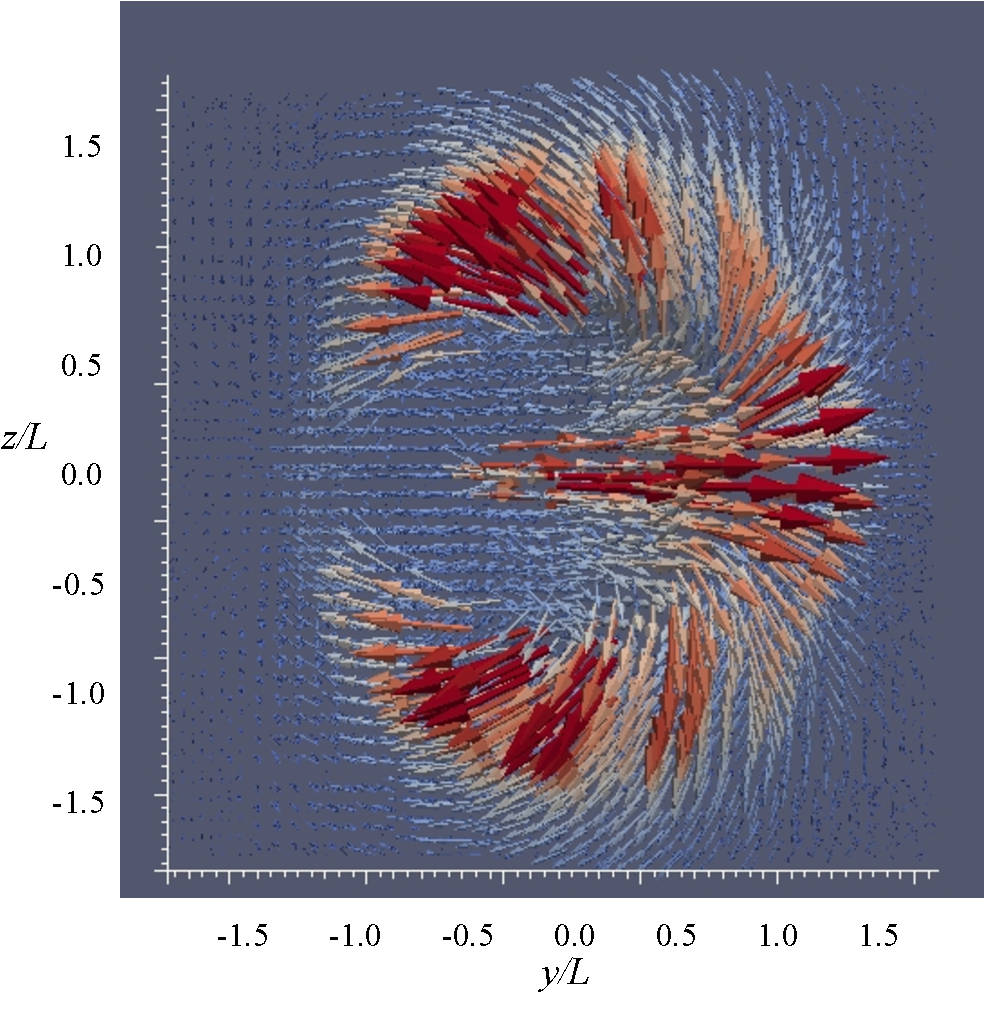
\includegraphics[width=12cm]{./figures/Fig_4_bb-crop.pdf}
\caption{All skyview map of current density with arrows 
observed from the lunar ground}\label{fig:4}
\end{figure}

In the current study, 
we are interested in the structure of the boundary layer current  
of the mini-magnetosphere.
In Figure \ref{fig:4} 
we plot arrows of total current density in a three-dimensional region 
consisting of an area from $-1.68L$ to $1.68L$ in the $yx$ plane
with the altitude range from 0 to $1.678L$ from the lunar surface.
The plot is identical to an all-sky view of the total current vectors
above the magnetic anomaly from the lunar surface.
The current density values are normalized to 
the solar wind ion density $J_\mathrm{0i}$.
The red arrows imply the current intensity of approximately four times $J_\mathrm{0i}$.
As shown in the figure, 
we find two symmetric structures of large rotational current 
created in the upper and lower regions 
with respect to the equatorial plane $z=0$.
In the low latitude region including the equator, 
intense current is found mostly along the right direction in the figure
which corresponds to the dawnward direction.
When we see the high latitude regions 
which correspond to the upper and lower regions in the figure,
however, the arrows turn around and change the direction to the duskside region. 
It seems that the current turns around in the counterclockwise direction 
in the upper region and the clockwise direction in the lower region.
In other words, the equator current flowing in the dawnward direction 
splits and turns around to each hemisphere.
In the high latitude region in each hemisphere around $|z/L|$ is around 1.0, 
the current tends to flow to the duskward direction which is opposite to the 
direction of the equator current.

%% - Figure 5-
\begin{figure}[t]
\centering
\noindent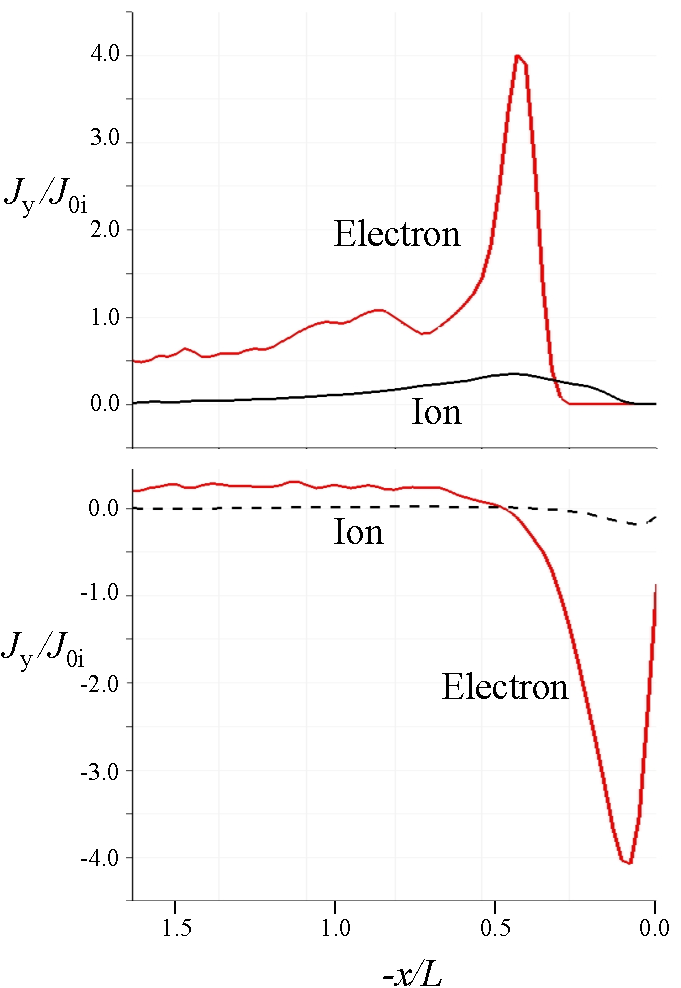
\includegraphics[width=12cm]{./figures/Fig_5_bb-crop.pdf}
\caption{Electron and ion current densities along $y=z=0$ and $y=0, z=L$ }\label{fig:5}
\end{figure}

To examine the detail of the boundary layer current, 
we decompose the total current into electron current 
and ion current as shown in Figure \ref{fig:5}. 
Panels (a) and (b) show the current intensities 
measured at the different latitudes $y=0, z=0$ and $y=0, z=L$, respectively.
The electron and ion current densities normalized to $J_\mathrm{0i}$ are 
indicated in red and black, respectively. 
As shown in the both panels, 
the ion current shown in black is much smaller than the electron current. 
It implies that the boundary layer current is dominated by the electron current. 
In panel (a), 
the current current has a peak of positive value. 
Considering the negative charge of the electron, 
electron flux points to the negative $y$ direction which is the duskward direction. 
In panel (b) corresponding to the high latitude region, on the other hand,  
we see a current peak with a negative value around $x=0.1L$ close to the lunar surface. 
In this case, the direction of the electron flux is the dawnward direction.  
Considering panels (a) and (b), we can clarify that the boundary layer current 
of the mini-magnetosphere dominantly consists of electrons and 
the directions of the electron flux are opposite to each other 
in the regions between the low and high latitudes. 
These signatures of the electron flux agree with the
turn-around current structure in the three-dimensional space 
as shown in Figure \ref{fig:4}.
To understand the structure of the boundary layer current, 
we next focus on electron flux in detail in different planes.

%%---  For Fig 6 and 7, we need to modify the contour maps --

%% - Figure 6-
\begin{figure}[h]
\centering
\noindent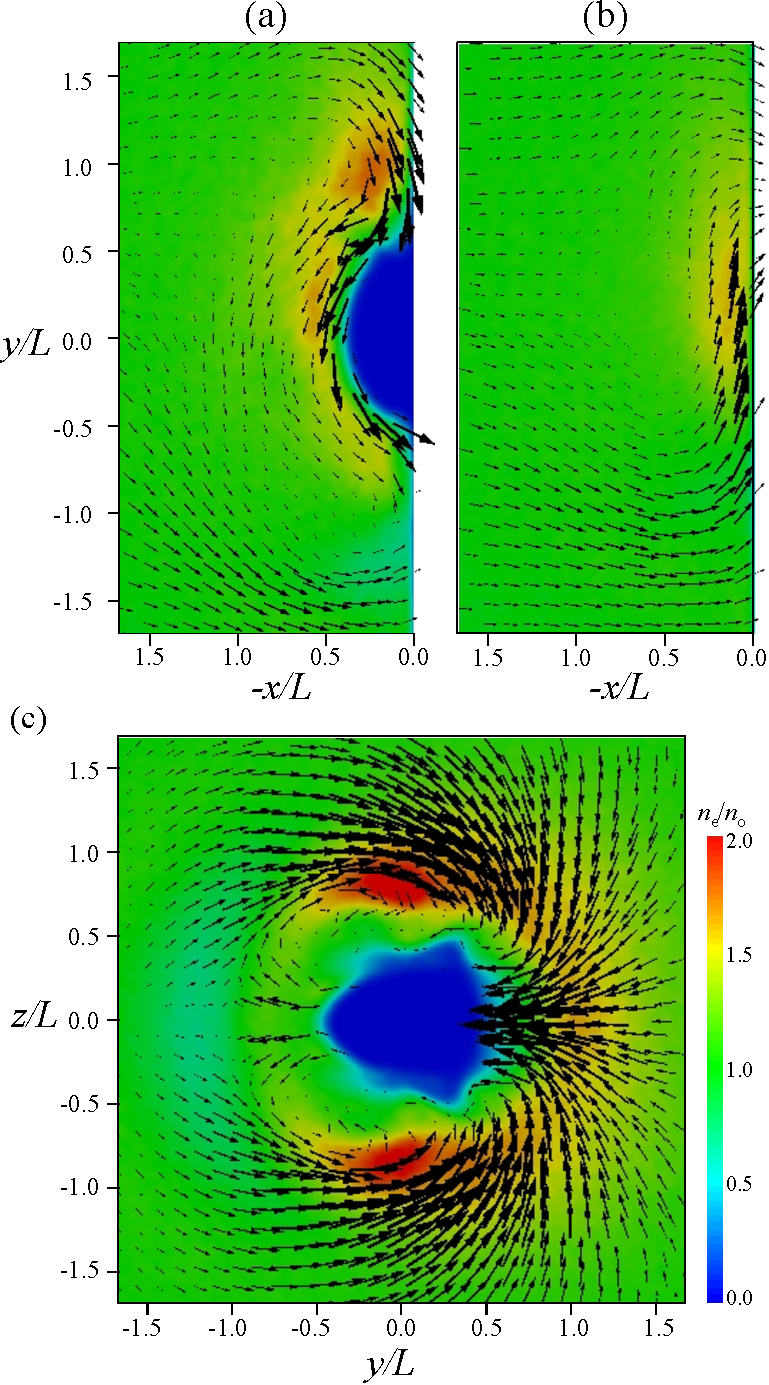
\includegraphics[width=12cm]{./figures/Fig_6_bb-crop.pdf}
\caption{Vector plots of electron current densities superimposed on the contour map 
of the electron density in the planes of (a) $z=0$, (b) $z=L$, (c) and $x=0.1L$.}\label{fig:6}
\end{figure}

Figure \ref{fig:6} shows arrows of the electron flux 
normalized to that in the unperturbed solar wind electron flux in different planes.
In each panel, contour map shown beneath the arrows indicates the electron density.
Panels (a) and (b) correspond to the profiles 
in the equatorial plane $z=0$ and a plane of $z=L$. 
Note that the direction of the arrows in Fig \ref{fig:6} is
different from that in Fig \ref{fig:4} because 
we plot the electron flux, not electron current.
In panel (a),  
we see asymmetric profile of the electron flux 
with respect to the line of $y=0$.
It seems that electrons dominantly enter the dawnside region 
and they stream along the boundary region of the high electron density
toward the duskside region.
It is interesting that the intense flux is found at the inner side of 
the peak density of electrons in the boundary region.
In panel (b) which shows the profile in the high latitude region, 
we also find an intense flux region close to the lunar surface.
It should be noted that the direction of the flux becomes 
opposite to the one found in panel (a) and points to the dawnward direction.
%This change of the flux direction basically agrees with 
%the total current profile shown in Fig \ref{fig:4}. 

Panel (c) shows the $yz$ components of the electron flux 
with arrows in $x=0.1L$, 
superimposed on the electron density contour map of the corresponding plane.
The panel corresponds to a cross-section of the mini-magnetosphere.
The contour map indicates an asymmetric density cavity 
surrounded by high density boundary layer which is also asymmetric.
These asymmetric density profiles were also discussed in the previous works
(\cite{Deca2014}).
As shown in panel (c)
a large convective structure of electron flux is found 
in the high density region in each hemisphere.
The direction of the electron flux is to the dawnside region at the high latitudes and
the flux turns around to the low latitude and converges to the dawnside region.
Then the flux streams into the equator toward the duskward direction.
Although not shown in panel (c), 
the electron flux converging to the equator flows 
along the inner edge of the boundary layer as shown in panel (a).
Considering the flux profile shown in panels (a),(b) and (c), 
it is found that solar wind electrons flowing 
to the high latitude boundary layer of the mini-magnetosphere
changes the direction to the dawnward direction 
near the lunar surface and converges down to the equator region 
and then the flow changes the direction to the duskward
along the inner boundary of the mini-magnetosphere in the equatorial plane.
This three-dimensional profile of the electron flux basically 
agrees with the all-sky view of the current density shown in Figure \ref{fig:4}.

%% - Figure 7-
\begin{figure}[h]
\centering
\noindent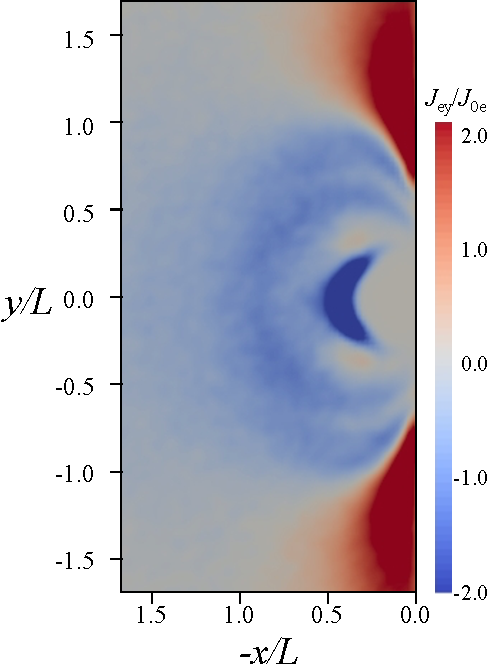
\includegraphics[width=10cm]{./figures/Fig_7_bb-crop.pdf}
\caption{Contour map of the $y$ component of the electron current density 
on the meridian plane $y=0$.}\label{fig:7} 
\end{figure}

To show the dependency of the direction of the electron flux on the latitude, 
we examine the $y$ component of the electron flux in a meridian plane at $y=0$.
Figure \ref{fig:7} shows a contour map for the intensity of 
the $y$ component of the electron flux.
As shown in the figure, 
positive values which implies the electron flux toward the dawnward direction
are found in the high latitude regions both in north and south hemispheres
near the polar regions.
In other regions, on the other hand, 
negative values are dominant as shown in blue, 
which implies that the electron flux is mostly toward the duskward direction. 
The most intense flux is found in the equator region as well as 
the high latitude regions, 
although the directions of the flux are opposite to each other.
We can confirm that this reverse of the flux at the different latitudes can 
cause a turn-around current structure connecting between the lower and higher latitudes 
as shown in the overview profile of the total current shown in Figure \ref{fig:4}.


\section{Discussions}

%% - Figure 8-
\begin{figure}
\centering
\noindent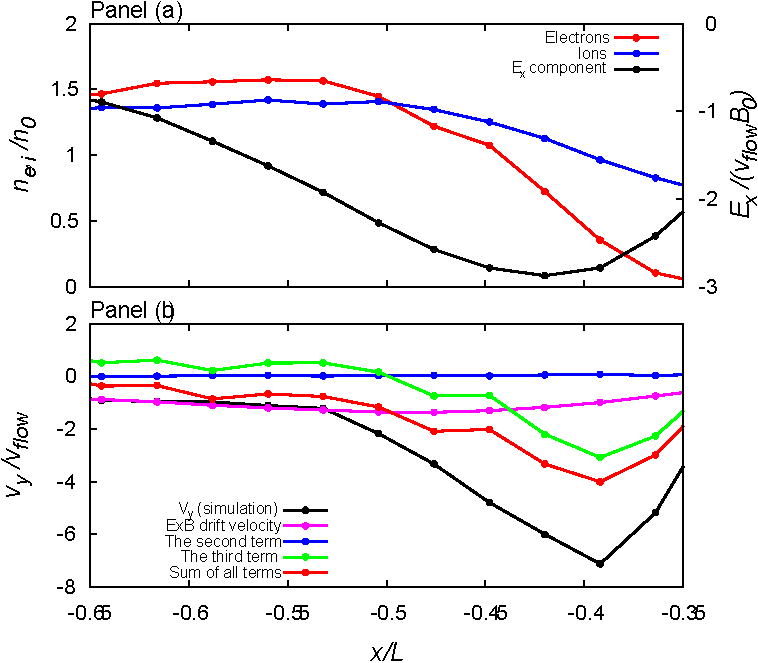
\includegraphics[width=15cm]{./figures/Fig_8_bb-crop.pdf}
\caption{
(a) Electron and ion density variation and $E_x$ intensity, and 
(b) $E \times B$ drift velocity obtained with the field values in the simulation (red curve), 
    $v_y$ of electrons estimated with the electron fluid equation (Eq (\ref{eqn:3}))
     by using the simulation data (blue curve) and  
    $v_y$ of electrons obtained with the particle data in the simulation (black curve),
  along $y=z=0$ in the region between $x/L = -0.65$ and $-0.35$. } 
\label{fig:8}
\end{figure}

We find that the boundary layer current of the mini-magnetosphere 
mainly consists of the electron flow. 
As shown in Figure \ref{fig:7}, 
the electron flux 
to the direction from the right-hand to the left-hand hemisphere
is dominant in the magnetic equator.
This flux is perpendicular to the dipole magnetic field. 
When $r_\mathrm{eL}$ is much smaller than $L$ as in the present case,
this perpendicular flux can be due to the drift motion of electrons.
Here, we further examine the electron dynamics in the magnetic equator.
In panel (a) of Figure \ref{fig:8} 
we show one-dimensional plots of the $x$ component of 
the electric field $E_x$ as well as
electron and ion densities measured along the line of $y=z=0$. 
$E_x$ and the densities are normalized to 
$v_\mathrm{flow} B_\mathrm{0}$ and $n_\mathrm{0}$, respectively.
These quantities are plotted in the region from $x/L = -0.65L$ to $-0.35L$
where the plasma density starts decreasing toward the lunar surface.
As shown in black in panel (a), 
$E_x$ has large negative value with 
a peak around at  $x/L = -0.42 $.
This intense electric field is caused by the density difference 
between electrons and ions in the boundary layer.
Particularly in the inner boundary layer 
corresponding to the region in the panel 
between $x/L = -0.5$  and $-0.35$, 
the electron density shown in red decreases and 
the ion density density in blue becomes dominant.
Since ions are less magnetized than electrons in the dipole field, 
they can approach the lunar surface.
This charge separation between ions and electrons
causes the intense electric field shown in black in the panel.
The resulting electric field points to the sunward direction
above the magnetic anomaly.
Considering that the dipole magnetic field points
to the negative $z$ direction in the magnetic equator,
the direction of the $E \times B$ drift velocity becomes 
along the negative $y$ direction 
which corresponds to the direction 
from the right-hand to the left-hand hemisphere.
We here examine if the intense electron flux observed in the magnetic equator
shown in Figure \ref{fig:7} can be explained by the drift motion of electrons
with the $E \times B$ velocity. 
In the following, 
we discuss the $v_y$ component of electrons along the line $y=z=0$.
Assuming that the electrons located in the boundary layer 
are almost magnetized and 
$r_\mathrm{eL}$ of those electrons is small enough in comparison 
to the structure of the boundary layer, 
we use the following fluid equation for electrons.
 
\begin{linenomath}
 \begin{equation}
%  m_\mathrm{e} n_\mathrm{e} \frac{d \mbox{\boldmath v}}{dt}
%    = q_\mathrm{e} n_\mathrm{e}(\mbox{\boldmath E} +
%      \mbox{\boldmath v} \times \mbox{\boldmath B}) - 
%      \nabla P_\mathrm{e}
  m_\mathrm{e} n_\mathrm{e} \frac{d \boldmath v}{dt}
    = q_\mathrm{e} n_\mathrm{e}(\boldmath E +
      \boldmath v \times \boldmath B) - 
      \nabla P_\mathrm{e}
 \label{eqn:1}
 \end{equation}
\end{linenomath}
where $P_\mathrm{e}$ denotes the electron pressure.
Note that Equation (\ref{eqn:1}) does not include the effect of 
the finite Larmor radius of the electron cyclotron motion (ECM)
because of fluid approximation.
When we assume the steady state, 
%$\partial{\mbox{\boldmath v}}/\partial{t} = 0 $ in the above equation, 
$\partial{\boldmath v}/\partial{t} = 0 $ in the above equation, 
the following equation is obtained for the $x$ component of
the electron velocity $v_x$.

\begin{linenomath}
 \begin{equation}
  m_\mathrm{e} n_\mathrm{e} v_\mathrm{x} \frac{\partial v_\mathrm{x}}{\partial x}
% = q_\mathrm{e} n_\mathrm{e} (E_x + v_y B_z) -  K T_\mathrm{e} \frac{\partial n_\mathrm{e}} {\partial x}
%%    = q_\mathrm{e} n_\mathrm{e} (E_x + v_y B_z) -  \nabla (n_\mathrm{e} K_\mathrm{B} T_\mathrm{e})
    = q_\mathrm{e} n_\mathrm{e} (E_x + v_y B_z) -  \nabla P_{e}.
 \label{eqn:2}
 \end{equation}
\end{linenomath}
Equation (\ref{eqn:2}) shows the electron force balances 
in the $x$ direction (\cite{Moritaka2012}).
From this relation, we can obtain $v_y$ as follows.
To distinguish from the simulation result, 
we refer the estimated $v_y$ as $v_{y-fld}$ hereafter.

%\begin{linenomath}
% \begin{equation}
%    n_\mathrm{e} K_\mathrm{B} T_\mathrm{e}  = \frac{1}{3} m_\mathrm{e}{v_\mathrm{th}}^2
% \end{equation}
%\end{linenomath}

\begin{linenomath}
 \begin{equation}
  v_{y-fld} = 
   - \frac{E_x}{B_z} 
   + \frac {m_\mathrm{e}}{q_\mathrm{e} B_z}v_x\frac{\partial v_x}{\partial x}
   + \frac{1}{q_\mathrm{e} n_\mathrm{e} B_z}\nabla P_{e}.
%%   + \frac{1}{q_\mathrm{e} n_\mathrm{e} B_z}\nabla (n_\mathrm{e} \frac{1}{3} m_\mathrm{e}{v_\mathrm{th}}^2)
%        =
%   - \frac{E_x}{B_z} 
%   + \frac {m_\mathrm{e}}{q_\mathrm{e} B_z}v_x\frac{\partial v_x}{\partial x}
%   + \frac{m_\mathrm{e}}{3 q_\mathrm{e} n_\mathrm{e} B_z}(n_\mathrm{e} \nabla {v_\mathrm{th}}^2 
%      + {v_\mathrm{th}^2} \nabla {n_\mathrm{e}})
 \label{eqn:3}
 \end{equation}
\end{linenomath}

% --- modify on 160824 @ Brown -----
In Equation (\ref{eqn:3}), 
the first term implies the $E \times B$ drift velocity and 
the second one represents the inertial effect. 
The third term implies the velocity caused 
by the spatial variation of the plasma pressure. 
By using the simulation data such as $B_z$, $E_x$, $n_\mathrm{e}$, and $v_x$
obtained at each grid point along $y=z=0$, 
we can estimate $v_{y-fld}$ with Equation (\ref{eqn:3}). 
In panel (b) of Figure \ref{fig:8}, 
the first, the second and the third terms in Equation (\ref{eqn:3}) are plotted 
in magenta, blue, and green, respectively.  
The sum of the three terms, which corresponds to $v_{y-fld}$,
is shown in red. 
As shown in panel (b) of Figure \ref{fig:8},
the second term which is the inertia term shown in blue is negligible 
in comparison with the other terms. 
In other words, $v_{y-fld}$ estimated with Equation (\ref{eqn:3}) is 
dominated by the first and third terms. 
In comparison, 
we plot the simulation result in black which is obtained 
by the average of the $v_y$ component of the electron particles 
located at each $x$ position along $y=z=0$.
Hereafter we refer this as $<v_{y-sim}>$. 

In the region between $x/L=-0.65$ and $-0.5$, 
the black, red and magenta curves seem to approximately agree to each other. 
This implies that the $<v_{y-sim}>$ of electrons in this region 
is mainly due to the $E \times B$ drift velocity shown in magenta
and can be estimated with the fluid theory. 
The term of the pressure gradient shown in green is almost zero 
in the same region.  

In the inner boundary layer between $x/L=-0.5$ and $-0.35$, 
however, 
$<v_{y-sim}>$ shown in black do not match the red curve
$v_{y-fld}$.
%
%
%To examine $v_y$ of electrons in the boundary layer current of the magnetosphere, 
%we show spatial variations of relevant physical quantities in \ref{fig:10} 
%such as the electron and ion densities $n_\mathrm{e}, n_\mathrm{i}$ and the $x$ component of 
%the electric field $E_x$ measured along the line of $y/L= z/L =0$.
%%In the second panel in \ref{fig:9}, 
%%we plot $v_y$ values evaluated in the above fluid equation by using the simulation data. 
%%between $x/L = -0.65$ and $-0.5$ 
%%in the simulation domain.
%Note that the $v_y$ data at $x/L= -0.37$ contains some ambiguity because of insufficient 
%number of electrons.  
Particularly the difference from the magenta curve representing 
the $E \times B$ drift velocity becomes large.
While $<v_{y-sim}>$ shown in black decreases,
the $E \times B$ drift velocity in magenta keeps almost the same values. 
As shown in panel (a), the intensity of $E_x$ becomes large 
in the corresponding region and the $E \times B$ drift velocity 
is also supposed to increase. 
However, the dipole magnetic field simultaneously becomes intense 
in the same region and eventually the $E \times B$ velocity 
takes almost the same values as shown in magenta.
On the other hand, 
$v_{y-fluid}$ shown in red can show the similar tendency to 
$<v_{y-sim}>$ shown in black.
Although the quantitative values do not match each other,
the qualitative trend that 
$v_y$ starts decreasing 
%in the region between $x/L =-0.5$ and $-0.4$ 
is commonly seen in the both curves.
This implies that the third term in Equation (\ref{eqn:3})
which is caused by the
pressure gradient needs to be considered in the region 
in the region between $x/L =-0.5$ and $-0.4$ 
where the electron density starts to decrease to zero. 

%-- up here modified on 2016/8/23 at Brown.
%-- from here modified on 2016/8/24 at Brown.

The issue is the quantitative difference between 
$v_{y-fluid}$ shown in red and $<v_{y-sim}>$ shown in black
particularly in the region between $x/L =-0.5$ and $-0.4$ 
where the electron density keeps decreasing toward the lunar surface.

%% - Figure 9-
\begin{figure}
\centering
\noindent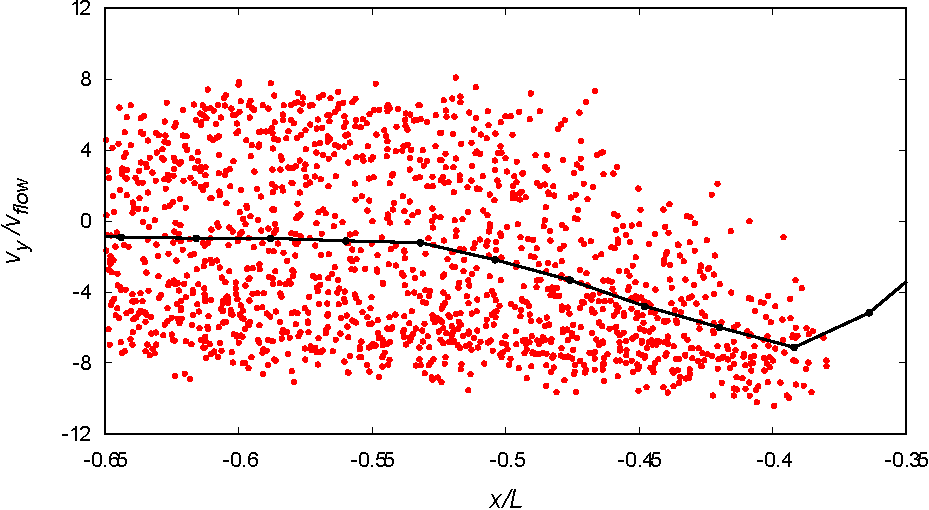
\includegraphics[width=15cm]{./figures/Fig_9_bb-crop.pdf}
\caption{
Electron phase diagram in the $x-v_{y}$ space in the region between $x/L =-0.65$ and $-0.35$
}
\label{fig:9}
\end{figure}

In order to understand this differece, 
we consider the finite Larmor radius of ECM 
which is solved in the PIC simulation, 
but no considered in Equation (\ref{eqn:3}).
In Figure \ref{fig:9}, 
we depict $v_y$ component of each electron versus $x$ with red dots
along the line of $y=z=0$.
As a reference, 
we superimpose the same curve of $<v_{y-sim}>$ 
as shown in the previous figure.
As clearly shown, 
electrons seem uniformly distributed 
in the region between $x/L =-0.65$ and $-0.5$.
However, in the region between $x/L =-0.5$ and $-0.4$ 
corresponding to the inner boundary layer, 
the disribution starts to converge 
and the center of the distribution decreases down to $-v_y/v_{flow}=8$. 
It should be noted that 
electrons located in the region between $x/L =-0.65$ and $-0.5$
are distributed in the $v_y$ axis with velocity width much larger 
than $v_{flow}$ as well as $v_{the}$ of the unperturbed plasma flow. 
The reason of the disribution spread will be discussed later.
%In the region between $x/L =-0.65$ and $-0.5$,
%$<v_{y-sim}>$ shown in black agrees with the $E times B$ drift velocity as stated above.
%The average $v_y$ shown in black accordingly decreases in this region.
In addition, it is very interesting that electrons
in the region between $x/L =-0.5$ and $-0.4$
have no positive $v_y$ which corresponds to the velocity directing from the
right-hand to the left-hand hemisphere.
The above-mentioned features of the electron distribution are closely
associated with EMC 
and are directly reflected in the curve of $<v_{y-sim}>$ shown in black.
%We will explain the detail below.
%This phenomenon cannot be predicted with the fluid approximation and can be
%very much associated with EMC around the dipole magnetic field.
%We will explain the detail below.

%%% up here we modified the manuscript on 2/26.

To see the effect of ECM in the boundary layer on the electron velocity distribution, 
we plot electrons in the $v_x-v_y$ phase space 
in Figure \ref{fig:10} for different locations along $y=z=0$.
Since the dipole magnetic field points to the negative $z$ direction perpendicular
to the magnetic equator, 
ECM is found in the $v_x-v_y$ phase space.
%% - Figure 10-
\begin{figure}
\centering
\noindent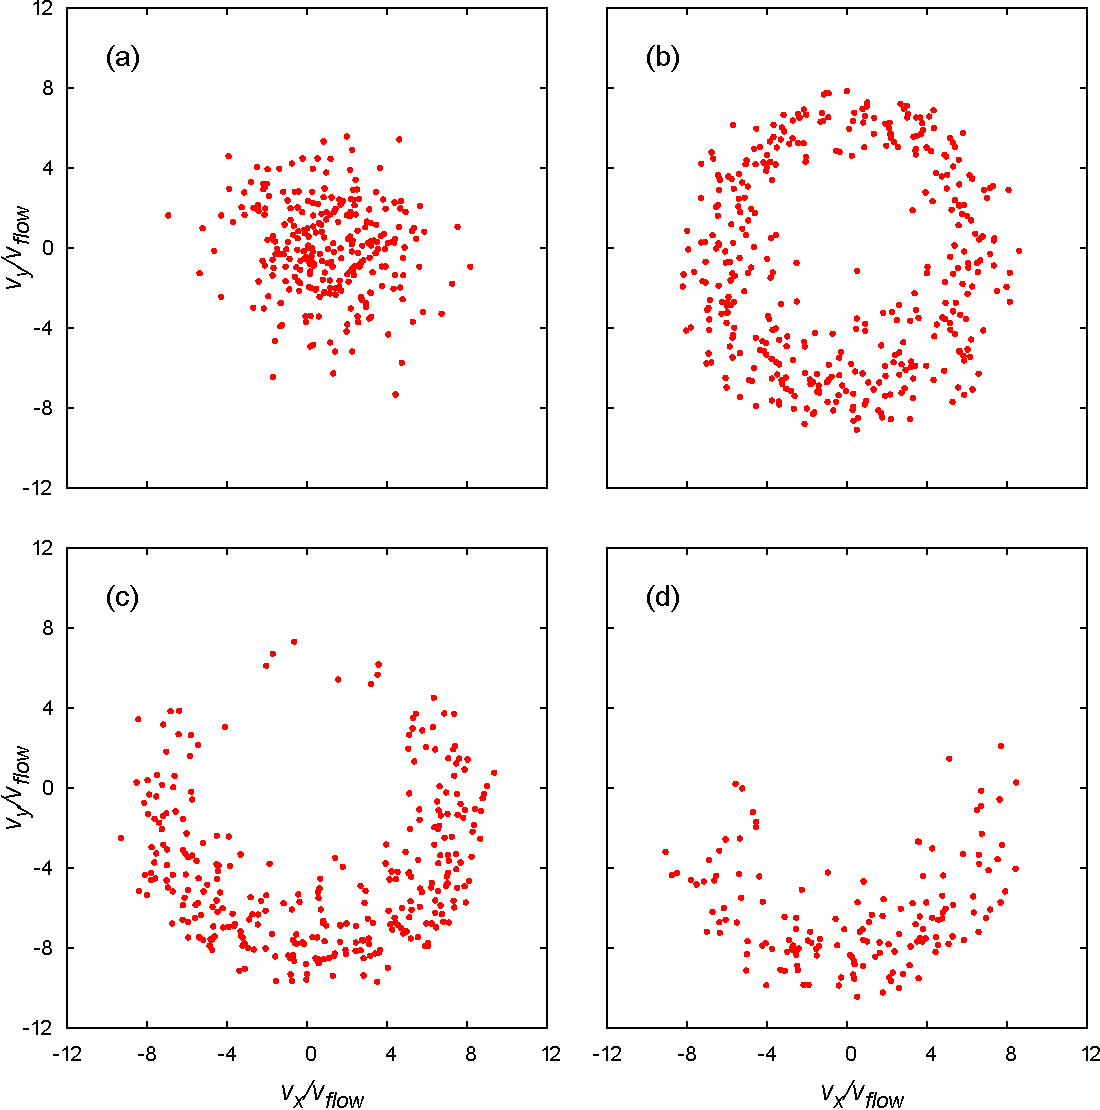
\includegraphics[width=15cm]{./figures/Fig_10_bb-crop.pdf}
\caption{Electron phase diagrams in the $v_{x}-v_{y}$ space in 
(a) the unperturbed region at $x/L = -5.0$ above the magnetic anomaly, 
(b) the region between $x/L =-0.59$ and $-0.53$  
(c) the region between $x/L =-0.48$ and $-0.42$ and
(d) the region between $x/L =-0.42$ and $-0.36$ }
\label{fig:10}
\end{figure}
Panel (a) shows a plot for the region of 
unperturbed electrons while the other panels
at different regions in the boundary layer between $x/L = -0.6$ and -0.4.
Panel (a) shows a unperturbed Maxwellian velocity distribution of electrons.
Since the unperturbed electrons have 
drift velocity of $v_{flow}$ toward the lunar surface,
the center of the distribution is shifted with $v_{flow}$ 
to the positive $v_x$ direction.
%
When those electrons enter the boundary layer, 
they start to be accelerated toward the lunar surface 
by $Ex$ induced by the charge separation 
shown in black curve in Panel (a) of Figure \ref{fig:8}.
We show a phase plot of electrons located between 
$x/L = -0.59$ and $-0.53$ in Panel (b) of Figure \ref{fig:10}.
It is clearly shown that the electrons accelerated by $E_x$ form 
a ring-like velocity distribution in the $v_x-v_y$ phase space.
%The electrons which are accelerated toward the negative $x$ direction 
%gain larger velocities and rotate with larger Larmor radius.
The maximum velocity of these electrons is approximately 
$|v|/v_\mathrm{flow} = 8$ which is much larger than 
the ambient thermal velocity $v_{the}/v_\mathrm{flow} = 2.4$ 
as well as the original flow velocity $v_\mathrm{flow}$.
This signature is also shown in the previous figure
in the region between $x/L =-0.65$ and $-0.5$.
Electrons entering the boundary layer
are accelerated by $E_x$ and start making the cyclotron motion 
with the much larger Larmor radius 
around the local magnetic dipole field. 
Panel (c) shows another phase plot for electrons located at the more inner boundary
layer between $x/L = -0.53$ and $-0.48$ 
where the electron density starts to decrease.
It should be stressed that 
the upper half of the velocity distribution is almost missing in Panel (c).
This non-uniform distribution agrees with the missing of the positive $v_y$ 
electrons found in Figure \ref{fig:9}.

The reason of this collaption of the ring distribution can be interprited 
as follows.
%Electrons entering to the boundary layer 
%is basically accelerated toward the lunar surface which is the negative $x$ direction 
%by the electric field induced by the charge separation.
As stated above, the electrons accelerated in the boundary layer
rotate around the local magnetic field with the larger Lamor radius.
Since this process continuously occurs for the electrons 
entering the boundary layer,
the electrons form a gyrotropic ring-distribution
%the electron velocity distribution becomes gyrotropic as shown in Panel (b) of \ref{fig:10}.
as shown in Panel (b) of Figure \ref{fig:10}.
In this region of the boundary layer, 
$<v_{y-sim}>$ agrees well with the $E \times B$ 
drift velocity because the electrons are gyrotropically 
distributed in the $v_x-V_y$ phase space.


%--- up to here, I modfied in the flight 2016/9/10 
%  need to think the reason why the electron density decreases.
%  


In the inner boundary layer, however, 
%when we approach the lunar surface, 
the electron density decreases because the intensity of the
local mangetic field becomes large.
%electrons with negative $v_x$ can move further to the inner boundary layer
At the most edge of the inner boundary layer,
due to ECM, electrons velocity vector points to the direction
of the right-hand to the left-hand hemisphere in the magnetic equator.
Assuming that the Larmor radius of the accelerated electrons
is larger than the region taken for Panel (c), 
electrons with positive $v_y$ are filtered out in the plot
and only the electrons moving to the direction
of the right-hand to the left-hand hemisphere, 
the negative $v_y$, are observed. 
%which corresponds to the negative $v_y$ in the phase space.
This is the reason why the electrons with positive $v_y$ 
are missing in the ring-distribution in Panel (c) of \ref{fig:10}.
This filtering due to ECM causes the maximum $v_y$ value around $x/L = -0.4$ as
shown in the black curves both in Figures \ref{fig:9} and \ref{fig:10}. 

% up here 16/8/25 noon @ brown
To confirm the above discussion on ECM 
at the edge of the inner boundary layer,
we plot a phase plot of the electrons located between 
$x/L = -0.48$ and $-0.36$ in Panel (d) of Figure \ref{fig:10}.
As shown in the panel, 
the most of the electrons have the maximum negative $v_y$ component 
with $|v|/v_\mathrm{flow}=8$. 
This implies that due to the spatial filtering of ECM 
most of the electrons located in the region 
are all pointing to the direction
of the right-hand to the left-hand hemisphere. 

Although the intensity of the dipole magnetic field changes depending on 
the distance from the lunar surface, 
the average intensity can be around $|B|=1.5$ in the inner boundary layer.
Assuming the averaged velocity of the accelerated electrons is 
$|v|/v_\mathrm{flow}=8$, as shown in Panel (d) of Figure \ref{fig:10} 
we can estimate that $r_\mathrm{eL}$ can be around $0.1L$.
%$ (0.4/1.5)/2.5 =0.1$.
%Then the diameter of the gyrating electrons in the corresponding region roughly becomes around $0.2L$.
This radius approximately agrees with the distance 
between $x/L = -0.5$ and -0.4 where
the electron density gradually decreases to zero.
Since this $r_\mathrm{eL}$ is larger than each region 
taken for Panels (b) to (c) of \ref{fig:10}, 
the velocity distribution of ECM spatially changes,
depending on the measurement point.
At the inner boundary layer,
it turns out that $<v_{y-sim}>$ differs from the $E \times B$ drift velocity
which is the guiding center velocity of ECM.
This maximum velocity of $v_y$ cannot be obtained with 
the pressure gradient effect which corresponds
to the third term of Equation (\ref{eqn:3}). 
The maximum velocity of $<v_{y-sim}>$ is only found at the edge of the
inner boundary layer and cannot be obtained without considering
the finite Larmor radius in ECM. 
This is one of the most significant finidings in the current study.

%The spatial width in which the electrons have negative $v_y$ component
%is approximately $0.1L$ which corresponds to the local electron gyroradius.

%%In Figure \ref{fig:8} we showed that at the most inner edge of the magnetosphere
%%there is a gap between the $v_y$ curve of electrons obtained in the simulation
%%and the one estimated with the electron fluid equation. 
%
%

Considering the above discussion including ECM, 
the maximum $v_y$ of the electrons found at the inner edge of the 
boundary layer is not due to the drift motion of the electron guiding center
but the ECM velocity accelerated by the local electric field. 
The width of the inner boundary layer with intense electron flux 
is approximately equivalent to the radius of local ECM, 
%This means that the width of the boundary layer current 
%is approximately equal to the radius of the local ECM,
which is not related to the ion dynamics at all.
This is another significant finding in the present study.

In the previous works done by other scientists \citep[e.g.][]{Deca2014},
it was stated that
the electron current at the mini-magnetosphere boundary is 
simply due to the electron drift motion of $E\times B$. 
This is true for the averaged electron behavior in the boundary layer region.
However, if we consider the electron kinetics and closely focus on the electron motion 
at the most inner edge of the boundary layer,
the maximum electron velocity does not agree with 
the conventional $E \times B$ drift velocity and it can be explained by the
cyclotron motion of the electrons accelerated by the local electric field. 

%
%
% up to here 2016/2/11 holiday around 17:00 at home
%
%

\section{Conclusions}
We studied the electron dynamics in the boundary layer current of 
a mini-magnetosphere created above a magnetic anomaly on the lunar surface 
by performing three-dimensional electromagnetic particle-in-cell simulations.
In this study, we focused on the following two aspects.
The first is the three-dimensional structure of 
the boundary layer current of the mini-magnetosphere. 
The second is the electron dynamics which dominates 
in the boundary layer current on the equatorial plane.
On the first aspect,
the simulations revealed  a turn-around current structure in the boundary layer in each hemisphere.
The solar wind electrons flowing 
to the high latitude boundary layer of the mini-magnetosphere
changes the direction to the dawnward direction 
near the lunar surface and converges down to the equator region 
and then the flow changes the direction to the duskward
along the inner boundary of the mini-magnetosphere in the equatorial plane.
This turn-around structure of the electron flow 
between the low-latitude and the high-latitude region is 
very characteristic in the mini-magnetosphere created above a magnetic anomaly.
On the second aspect,
%Regarding the second point of this study, 
the simulations revealed the mechanism of the electron flux in the equatorial plane. 
We examined the detail of the electron dynamics including the electron cyclotron motion,
and found the maximum electron velocity in the most inner region of 
the magnetosphere where the electron density gradually decreases to zero.
We clarified that the maximum electron velocity
is due to the electron cyclotron motion itself, 
not the drift motion of the electrons.
We also confirmed that the width of the boundary current layer 
is approximately equal to the radius of the local electron cyclotron motion.
The study also suggests that, in order to understand the electron current in the boundary of the mini-magnetosphere, 
 the finite Larmor radius of electrons must be included in the model.

%The maximum electron velocity found at the edge of the boundary region
%can be explained with the gyromotion of the electrons
%accelerated by the local $E$ field in the boundary region.
%The width of the electron current layer is approximately equal to 
%the diameter of the electron gyration.
As a future work, we plan to further study the %mechanism of the 
electron dynamics in the high-latitude region which has the opposite direction to that in the equator.
Unlike the situation on the equator, the direction of the dipole magnetic field is not simply 
along the north-south direction in the high latitude region.  
If the electron flux is also dominated by the $E \times B$ drift motion, 
one then needs to examine the relative angle between
the local $E$-field and the dipole magnetic field.
We also need to consider the electron kinetic effect such as the finite 
$r_\mathrm{eL}$ to explain the maximum electron velocity in the high latitude region, 
%which is left as a future work.
%As exmined in the present study, the intense electron flux can be due to 
%the electron gyration at the edge of the magnetosphere in the high-latitude region.
%Since the size of the magnetosphere is much smaller than the Earth's magnetosphere, 
%electron kinetics becomes important to understand the physics in the mini-magnetosphere.


%%%%%%%%%%%%%%%%%%%%%%%%%%%%%%%%
%% Optional Appendix goes here
%
% \appendix resets counters and redefines section heads
% but doesn't print anything.
% After typing \appendix
%
%\section{Here Is Appendix Title}
% will show
% Appendix A: Here Is Appendix Title
%
%%%%%%%%%%%%%%%%%%%%%%%%%%%%%%%%%%%%%%%%%%%%%%%%%%%%%%%%%%%%%%%%
%
% Optional Glossary or Notation section, goes here
%
%%%%%%%%%%%%%%
% Glossary is only allowed in Reviews of Geophysics
% \section*{Glossary}
% \paragraph{Term}
% Term Definition here
%
%%%%%%%%%%%%%%
% Notation -- End each entry with a period.
% \begin{notation}
% Term & definition.\\
% Second term & second definition.\\
% \end{notation}
%%%%%%%%%%%%%%%%%%%%%%%%%%%%%%%%%%%%%%%%%%%%%%%%%%%%%%%%%%%%%%%%
%
%  ACKNOWLEDGMENTS

\begin{acknowledgments}
This work was supported by JSPS KAKENHI Grant Number 23340148. 
Computation resources have been provided by the KDK of Kyoto University
and Pi-computer of ECCSE in Kobe University.
\end{acknowledgments}

%% ------------------------------------------------------------------------ %%
%%  REFERENCE LIST AND TEXT CITATIONS
%
% Either type in your references using
% \begin{thebibliography}{}
% \bibitem{}
% Text
% \end{thebibliography}
%
% Or,
%
% If you use BiBTeX for your references, please use the agufull08.bst file (available at % ftp://ftp.agu.org/journals/latex/journals/Manuscript-Preparation/) to produce your .bbl
% file and copy the contents into your paper here.
%
% Follow these steps:
% 1. Run LaTeX on your LaTeX file.
%
% 2. Make sure the bibliography style appears as \bibliographystyle{agufull08}. Run BiBTeX on your LaTeX
% file.
%
% 3. Open the new .bbl file containing the reference list and
%   copy all the contents into your LaTeX file here.
%
% 4. Comment out the old \bibliographystyle and \bibliography commands.
%
% 5. Run LaTeX on your new file before submitting.
%
% AGU does not want a .bib or a .bbl file. Please copy in the contents of your .bbl file here.

\bibliographystyle{agufull08}
\bibliography{luna_151002}

%%\begin{thebibliography}{}
%\providecommand{\natexlab}[1]{#1}
%\expandafter\ifx\csname urlstyle\endcsname\relax
%  \providecommand{\doi}[1]{doi:\discretionary{}{}{}#1}\else
%  \providecommand{\doi}{doi:\discretionary{}{}{}\begingroup
%  \urlstyle{rm}\Url}\fi
%
%\bibitem[{\textit{Atkinson and Sloan}(1991)}]{AtkinsonSloan}
%Atkinson, K., and I.~Sloan (1991), The numerical solution of first-kind
%  logarithmic-kernel integral equations on smooth open arcs, \textit{Math.
%  Comp.}, \textit{56}(193), 119--139.
%
%\bibitem[{\textit{Colton and Kress}(1983)}]{ColtonKress1}
%Colton, D., and R.~Kress (1983), \textit{Integral Equation Methods in
%  Scattering Theory}, John Wiley, New York.
%
%\bibitem[{\textit{Hsiao et~al.}(1991)\textit{Hsiao, Stephan, and
%  Wendland}}]{StephanHsiao}
%Hsiao, G.~C., E.~P. Stephan, and W.~L. Wendland (1991), On the {D}irichlet
%  problem in elasticity for a domain exterior to an arc, \textit{J. Comput.
%  Appl. Math.}, \textit{34}(1), 1--19.
%
%\bibitem[{\textit{Lu and Ando}(2012)}]{LuAndo}
%Lu, P., and M.~Ando (2012), Difference of scattering geometrical optics
%  components and line integrals of currents in modified edge representation,
%  \textit{Radio Sci.}, \textit{47},  RS3007, \doi{10.1029/2011RS004899}.

%%\end{thebibliography}

%Reference citation examples:

%...as shown by \textit{Kilby} [2008].
%...as shown by {\textit  {Lewin}} [1976], {\textit  {Carson}} [1986], {\textit  {Bartholdy and Billi}} [2002], and {\textit  {Rinaldi}} [2003].
%...has been shown [\textit{Kilby et al.}, 2008].
%...has been shown [{\textit  {Lewin}}, 1976; {\textit  {Carson}}, 1986; {\textit  {Bartholdy and Billi}}, 2002; {\textit  {Rinaldi}}, 2003].
%...has been shown [e.g., {\textit  {Lewin}}, 1976; {\textit  {Carson}}, 1986; {\textit  {Bartholdy and Billi}}, 2002; {\textit  {Rinaldi}}, 2003].

%...as shown by \citet{jskilby}.
%...as shown by \citet{lewin76}, \citet{carson86}, \citet{bartoldy02}, and \citet{rinaldi03}.
%...has been shown \citep{jskilbye}.
%...has been shown \citep{lewin76,carson86,bartoldy02,rinaldi03}.
%...has been shown \citep [e.g.,][]{lewin76,carson86,bartoldy02,rinaldi03}.
%
% Please use ONLY \citet and \citep for reference citations.
% DO NOT use other cite commands (e.g., \cite, \citeyear, \nocite, \citealp, etc.).

%% ------------------------------------------------------------------------ %%
%
%  END ARTICLE
%
%% ------------------------------------------------------------------------ %%
\end{article}
%
%
%% Enter Figures and Tables here:
%
% DO NOT USE \psfrag or \subfigure commands.
%
% Figure captions go below the figure.
% Table titles go above tables; all other caption information
%  should be placed in footnotes below the table.
%
%----------------
% EXAMPLE FIGURE
%
 %\begin{figure}
 %\noindent\includegraphics[width=20pc]{samplefigure.eps}
 %\caption{Caption text here}
 %\label{figure_label}
 %\end{figure}
%
% ---------------
% EXAMPLE TABLE
%
%\begin{table}
%\caption{Time of the Transition Between Phase 1 and Phase 2\tablenotemark{a}}
%\centering
%\begin{tabular}{l c}
%\hline
% Run  & Time (min)  \\
%\hline
%  $l1$  & 260   \\
%  $l2$  & 300   \\
%  $l3$  & 340   \\
%  $h1$  & 270   \\
%  $h2$  & 250   \\
%  $h3$  & 380   \\
%  $r1$  & 370   \\
%  $r2$  & 390   \\
%\hline
%\end{tabular}
%\tablenotetext{a}{Footnote text here.}
%\end{table}



%%%%%%%%%%%%%%%%%%%%%%%%%%%%%%%%
%% Optional Appendix goes here
%
% \appendix resets counters and redefines section heads
% See below for how to make sideways figures or tables.

\end{document}
